% PAPER A (conference version): trust-filtered Byzantine-robust FL for grayhole detection in VANETs.
% Published FIRST; Paper B (../B_journal_extension/) is its journal extension.
% Scope: v3 network + FL pipeline only, incl. slow-recovery trust + warm-up (on-off defence). Neighbourhood-relative
% trust, per-vehicle warm-up/handover, volatility, cross-layer check, RSU uploads, PQ and VeReMi are reserved for Paper B.
% Numbers: tab:main from make_tables.py; other numbers in dataset_fl-training-v3-ring/report.txt, report_harder.txt,
% report_paperA.txt; figures: make_figs.py; per-round check: perround_check.py.
% Target: IEEE VCC 2027 (Virtual Conference on Communications, ComSoc, fully virtual, 2-4 Mar 2027).
% Deadline 27 Nov 2026 (extended; CFP page still says 6 Nov), EDAS, max 6 pages IEEE double column (longer = rejected
% without review), notification 18 Jan 2027, camera-ready 8 Feb 2027. CONFIRM: blind review or not.
% Fallback if rejected: VTC2027-Fall (Osaka, hybrid with virtual presentation), deadline 1 Feb 2027.
% Status: submission draft, 2026-11-10.
\documentclass[conference]{IEEEtran}
\usepackage{amsmath,amssymb,amsthm}
\usepackage{graphicx}
\usepackage{booktabs}
\usepackage{multirow}
\usepackage{array}
\usepackage{cite}
\usepackage{xcolor}
\usepackage[hidelinks]{hyperref}

\newtheorem{proposition}{Proposition}
\newtheorem{corollary}{Corollary}
\newcommand{\rsurv}{\rho_{\mathrm{surv}}}
\newcommand{\todo}[1]{\textcolor{red}{[TODO: #1]}}

\begin{document}

\title{Watchdog Trust for Byzantine-Robust Federated Learning in VANETs: A Measurable Breakdown Condition, and Where It Fails}

\author{\IEEEauthorblockN{Shahoriar Islam Khan\IEEEauthorrefmark{1}, Mazharul Islam\IEEEauthorrefmark{1}, and
Umme Habiba Tisha\IEEEauthorrefmark{2}}% \todo{confirm author order}
\IEEEauthorblockA{\IEEEauthorrefmark{1}Department of Computer Science and Engineering, Khulna University of Engineering \& Technology,
Khulna, Bangladesh}
\IEEEauthorblockA{\IEEEauthorrefmark{2}Department of Computer Science and Engineering, North Western University, Khulna, Bangladesh\\
Corresponding author: imazharul175@gmail.com}}

\maketitle

\begin{abstract}
Byzantine-robust aggregation protects federated learning (FL) only while attackers are a minority of the updates
in a round. In vehicular networks attackers are rare on the road, but their share among the updates of one round
can still be large: rounds are local, small and biased towards vehicles that stay. Vehicles that poison a shared
detector often also misbehave on the network, where neighbours can observe them. We study a filter that scores
each vehicle by watchdog observations of its packet forwarding and discards low-trust updates before robust
aggregation. The filter turns the breakdown point of the aggregator into a function of two measurable rates, the
attacker pass rate $\beta$ and the honest rejection rate $\gamma$: robust aggregation holds while
$\beta/(1-\gamma) < (1-\rho)/\rho$. In ns-3 simulations with grayholes that really drop transit packets, non-IID
clients and vehicle-disjoint evaluation, the filter raises no false alarms and costs no accuracy when attackers
are rare (0--10\%), and under sign-flip, label-flip and ALIE poisoning it keeps every trust-filtered rule at the no-attack F1 up to a 70\%
attacker share, while median, trimmed mean and Krum each fail against at least one attack from 40--60\%. The
condition predicts whether trust-filtered median survives in all 56 settings we test. It also maps the limits: weak and on-off grayholes
raise $\beta$; slow trust recovery with a 30~s observation period repairs the on-off case, and a per-round analysis
explains why the observation period is needed. Poisoners that forward honestly defeat the filter.
\end{abstract}

\begin{IEEEkeywords}
Federated learning, VANET, grayhole attack, Byzantine robustness, trust management, watchdog, ns-3.
\end{IEEEkeywords}

% =====================================================================================
\section{Introduction}
% =====================================================================================

Grayhole attacks, in which a vehicle that should relay packets silently drops some of them, remain a practical
threat to multi-hop vehicular ad hoc networks (VANETs)~\cite{vanderheijden2019}. Learning-based detectors trained on network features can
identify such vehicles, and federated learning (FL)~\cite{mcmahan2017} lets vehicles train a shared detector without
uploading their observations. FL is itself exposed to poisoning by the same malicious vehicles~\cite{fang2020local,tolpegin2020}. Byzantine-robust
rules such as Krum~\cite{blanchard2017}, coordinate-wise median and trimmed mean~\cite{yin2018} tolerate poisoned
updates only while attackers are a minority of the updates they aggregate, and their non-IID
refinements~\cite{karimireddy2022} need a margin below that.

Attackers are rare on a real road, so why worry about majorities? Because the share that matters is the share
\emph{in a round}, not on the road. Vehicular FL rounds are local (the vehicles near one roadside unit or in one
area), often small, and biased towards vehicles that stay in coverage, which a parked
attacker does and a passing honest vehicle does not. A few colluding attackers can therefore be a majority of one
round while being a few percent of all traffic, and random client sampling alone produces such rounds~\cite{allouah2024}.

Vehicular FL also has a resource that generic FL lacks: the network is observable. A vehicle that drops packets it
should forward can be caught by its neighbours with a watchdog~\cite{marti2000}. Vehicular FL schemes already weight
or select clients by reputation~\cite{su2025electronics,titsrc2026,vnc2024hfl,iwcmc2025trust,vnc2026sdv}, but they
compute it from the model updates or from interaction history, which shares the blind spots of the aggregator. We
ask: \emph{if trust comes from observable network behaviour, when does it keep Byzantine-robust FL working, at what
cost when attackers are rare, and where does it stop?} We answer with a pipeline built to avoid shortcuts: attackers
really drop transit packets in ns-3, features come from what a watchdog can actually overhear (including false
accusations from collisions and mobility), the threshold is label-free, trust uses only past observations, clients
are non-IID, and evaluation is vehicle-disjoint 3-fold cross-validation.

\textbf{Contributions.}
\begin{enumerate}
\item \emph{A breakdown condition in observable quantities.} The filter maps the attacker share $\rho$ to an
aggregated share $\rsurv$ that depends only on its pass and rejection rates (Proposition~\ref{prop:cond}); the
breakdown point becomes $(1-\gamma)/(1-\gamma+\beta)$, 0.95 for the filter we measure. $\rsurv < 1/2$ predicts the
survival of trust-filtered median in all 56 settings (Fig.~\ref{fig:phase}).
\item \emph{Robustness that does not depend on the poisoning attack, at no accuracy cost when attackers are rare.}
With 0--10\% attackers the filter matches unfiltered training and raises no false alarms; up to a 70\% share it
keeps all trust-filtered rules at the no-attack F1 under sign-flip, label-flip and ALIE~\cite{baruch2019}, whereas each unfiltered robust rule fails
against at least one of them.
\item \emph{A map of failure modes and two fixes.} Weak and on-off grayholes raise $\beta$; slow trust recovery with
a short observation period restores the on-off case, and a per-round analysis of 1{,}260 runs shows that failures
the pooled condition misses happen before attackers are detected. Honest-forwarding poisoners defeat the filter,
which then amplifies them.
\end{enumerate}

% =====================================================================================
\section{Related Work}
% =====================================================================================

\textbf{Byzantine-robust FL.} Krum~\cite{blanchard2017} selects the update closest to its neighbours; median and
trimmed mean~\cite{yin2018} act per coordinate; bucketing~\cite{karimireddy2022} averages random groups first to
reduce heterogeneity. All assume an honest majority among aggregated updates; ALIE~\cite{baruch2019} evades them
even then, and client subsampling can create Byzantine-majority rounds~\cite{allouah2024}. Defences that
tolerate an attacker majority need trusted data at the server: Zeno~\cite{xie2019zeno} scores updates on a
validation set and FLTrust~\cite{cao2021fltrust} on a clean root dataset, while FLAME~\cite{nguyen2022flame}
clusters and clips updates under an honest majority. Our filter needs no server data; its signal is the network.

\begin{table}[t]
\caption{Trust in vehicular FL: where the score comes from and what is analysed.}
\label{tab:rw}
\centering
\footnotesize
\setlength{\tabcolsep}{2.5pt}
\begin{tabular}{@{}l>{\raggedright\arraybackslash}p{0.40\columnwidth}c>{\raggedright\arraybackslash}p{0.17\columnwidth}c@{}}
\toprule
Work & Trust signal & Indep.$^a$ & Evaluation & Breakdown$^b$\\
\midrule
\cite{su2025electronics} & Reputation from FL contributions & -- & IoV sim. & --\\
\cite{titsrc2026} & Communication behaviour, model transmissions & partly & IoV sim. & --\\
\cite{iwcmc2025trust} & Reputation, context, resources & partly & MNIST & --\\
\cite{vnc2024hfl} & Accuracy, contribution frequency, anomalies & -- & HFL sim. & --\\
\cite{vnc2026sdv} & Update consistency, anomaly deviation & -- & VeReMi & --\\
\midrule
Ours & Watchdog-observed packet forwarding & \checkmark & ns-3, real drops & \checkmark\\
\bottomrule
\end{tabular}\\[2pt]
\raggedright\scriptsize $^a$Signal independent of the model updates. $^b$Quantifies how filter errors ($\beta$,
$\gamma$) reach the aggregator and where it breaks.
\end{table}

\textbf{Reputation and trust in vehicular FL.} Trust management in VANETs is surveyed in~\cite{hussain2021trust},
and evicting misbehaving vehicles in~\cite{raya2007eviction}. Reputation-based selection with blockchain~\cite{su2025electronics},
trust-aware client selection with mobility and channel context~\cite{titsrc2026,iwcmc2025trust}, anomaly records in
hierarchical FL~\cite{vnc2024hfl} and update-consistency trust~\cite{vnc2026sdv} compute trust from model updates,
contribution history or link reliability, usually assume an attacker minority (at most 45\% in~\cite{su2025electronics}),
and do not quantify how the filter's errors reach the aggregator (Table~\ref{tab:rw}). Our trust comes from an
independent channel, network forwarding, and we give the exact propagation.

\textbf{Watchdogs.} Overhearing whether a relay forwards a packet is the classic defence against selective
forwarding~\cite{marti2000}; its false positives and negatives under collisions and mobility~\cite{cocowa2015} are
what make $\gamma > 0$ here, and on-off attacks against trust are known~\cite{sun2008onoff,bdpc2026}. We measure both inside FL.

% =====================================================================================
\section{System and Threat Model}
\label{sec:model}
% =====================================================================================

$N$ vehicles form a multi-hop VANET with AODV routing~\cite{rfc3561}. Each runs a watchdog and periodically reports its
observations; a server (e.g., at the edge) turns the reports into per-vehicle trust and coordinates FL rounds in
which vehicles train the shared detector and upload their models. We write $\rho$ for the attacker share among the
vehicles of an FL round. On the road $\rho$ is small; locally or in a round it can be large (Section~I). We do not model how
rounds become attacker-heavy; we evaluate the filter over round-level shares from 0 to 0.7.

Attackers are \emph{aligned}: each acts as a grayhole, dropping transit data packets with probability $p_d$ while
taking part normally in route discovery, and poisons its FL updates. We consider one data-poisoning and two
model-poisoning attacks: under \emph{label-flip}~\cite{tolpegin2020} each attacker trains on its data with every label inverted; under
\emph{sign-flip} each sends $w_g - \lambda (w - w_g)$, where $w_g$ is the global model, $w$ its locally trained model
and $\lambda = 5$; under non-omniscient \emph{ALIE}~\cite{baruch2019} all send $\mu - z\sigma$, the per-coordinate mean
minus $z$ standard deviations of the attackers' own honest updates. Harder network behaviours
are \emph{weak} grayholes ($p_d \in \{0.2, 0.3\}$), \emph{on-off} grayholes (drop 90\% for 10~s, forward honestly for
20~s, random phase), and \emph{decoupled} poisoners drawn from vehicles that forward honestly.

\textbf{Out of scope.} Attackers hold one identity each (no Sybil identities), do not forge route replies (a blackhole
that attracts routes is easier to detect), and do not tune their dropping to the threshold; denial of service and
inference attacks are not considered. Trust-aware attackers, Sybil identities and authenticated uploads are studied
in follow-up work.

% =====================================================================================
\section{Trust-Filtered Aggregation}
\label{sec:method}
% =====================================================================================

\textbf{Watchdog.} When vehicle $A$ hands a data frame to relay $X$ (network destination not $X$), it opens an entry;
the entry counts as forwarded if $A$ decodes $X$ re-transmitting the same packet within 1~s. A watchdog cannot tell a
drop from a missed overhearing, so honest vehicles score below one. Per vehicle and second we export cumulative
counters (relay requests, overheard forwards, route requests received and rebroadcast, packets and bytes, delay,
neighbours); ground truth goes only to a separate summary.

\textbf{Windowed trust.} At round time $t$ the trust of vehicle $v$ is $T_v = 0.7 f_v + 0.3 r_v$, with $f_v$ its
overheard forwarding ratio and $r_v$ its route participation (route requests rebroadcast over received), both from
counter differences over $(t - W, t]$, $W = 10$~s. A ratio with fewer than five events keeps its last value;
never-observed vehicles are accepted. As a slow-recovery variant, \emph{trust memory} $M$ takes the minimum windowed
trust over $(t - M, t]$, so a vehicle caught dropping stays suspect for $M$ seconds (slowed recovery after
misbehaviour is also used in~\cite{titsrc2026}; we measure its effect on $\beta$ and on the aggregator); with a \emph{warm-up} $\tau_w$,
updates are aggregated only after trust has observed the network for $\tau_w$ seconds.

\textbf{Label-free threshold.} Each round a two-component Gaussian mixture is fitted to the trust values and the low
component is rejected; if the Bayesian information criterion~\cite{schwarz1978} prefers one component, all vehicles are accepted.

\textbf{Aggregation.} Kept updates are combined by trust- and size-weighted averaging (Trust-FLAD, TF), Krum
(TF+Krum, $f = \lfloor n/4 \rfloor$), coordinate-wise median (TF+Median) or bucketed variants (bucket size 2).

% =====================================================================================
\section{When Does the Filter Restore Robustness?}
\label{sec:analysis}
% =====================================================================================

Let $\beta$ be the probability that the filter keeps an attacker and $\gamma$ the probability that it rejects an
honest vehicle. The attacker share among aggregated updates is
\begin{equation}
\rsurv = \frac{\rho\beta}{\rho\beta + (1-\rho)(1-\gamma)}.
\label{eq:surv}
\end{equation}

\begin{proposition}
\label{prop:cond}
$\rsurv < 1/2$ if and only if $\beta/(1-\gamma) < (1-\rho)/\rho$. Hence a rule that is robust while attackers are a
minority of its inputs stays robust after the filter for every $\rho < \rho^* = (1-\gamma)/(1-\gamma+\beta)$.
\end{proposition}
\begin{proof}
$\rsurv < 1/2 \iff \rho\beta < (1-\rho)(1-\gamma)$; solve for $\rho$.
\end{proof}

The left side depends only on how well network behaviour separates attackers from honest vehicles, the right side
only on the attacker share. With $\beta = 0.05$ and $\gamma = 0.10$, $\rho^* = 0.95$; with $\beta = 0.5$ (on-off
attackers) $\rho^* = 0.65$. Three remarks qualify the condition. (i) $\beta$ rises with $\rho$ when separation is
weak, because the honest reference population shrinks. (ii) For rules that need a margin (Krum, bucketing)
$\rsurv < 1/2$ is necessary, not sufficient; Krum can also survive $\rsurv > 1/2$ when poisoned updates are scattered
outliers. (iii) $\beta$ and $\gamma$ are run averages: an attacker passes until the watchdog has seen it misbehave, so
the condition describes the filter after a detection transient (Section~\ref{sec:perround}).

% =====================================================================================
\section{Simulation Setup}
\label{sec:setup}
% =====================================================================================

\textbf{Network.} ns-3.42~\cite{riley2010ns3}; 50 vehicles on a 2~km two-lane ring road at 20--30~m/s (constant density, no partitions);
IEEE 802.11a at 6~Mb/s, unit-disk propagation at 250~m, AODV; 30 UDP flows (512~B, 50~kb/s) between random pairs;
100~s per run. Attackers are a seeded random subset and drop transit data in a routing layer above AODV, leaving the
control plane untouched. Packet delivery is 0.90 without attackers and 0.44--0.82 with $p_d = 0.5$; the watchdog
forwarding ratio averages 0.93 for honest vehicles and 0.45 for grayholes.

\textbf{Learning.} The detector is an MLP (16 features, 32--16--1) that classifies a vehicle-second as attacker or
not. A client's data are the rows of the vehicles in its radio range (observed, non-IID clients). Vehicles are split
into three stratified folds whose rows are held out from all clients; predictions are pooled so every vehicle is
tested once. FL runs 20 rounds of 3 local epochs (Adam, learning rate 0.01, batch 128). Attacker shares
$\rho \in \{0, 0.04, 0.1, 0.2, \dots, 0.7\}$ (0 to 35 of 50 vehicles), five seeds each. We report F1 of the attacker
class against the ceiling, FedAvg without poisoning on the same network. Code and data: \url{https://github.com/MAZHAR1807102/watchdog-trust-fl-vanet}.

% =====================================================================================
\section{Results}
\label{sec:results}
% =====================================================================================

\begin{table*}[t]
\caption{F1 by attacker share, $p_d = 0.5$ (mean of 5 seeds, pooled 3-fold; 40\% and 60\% omitted for space,
quoted in the text). TF = trust-filtered; $\beta$, $\gamma$ of the filter.}
\label{tab:main}
\centering
\setlength{\tabcolsep}{4pt}
\begin{tabular}{l|ccccc|ccccc}
\toprule
& \multicolumn{5}{c|}{Sign-flip ($\lambda = 5$)} & \multicolumn{5}{c}{Label-flip}\\
Rule & 10\% & 20\% & 30\% & 50\% & 70\% & 10\% & 20\% & 30\% & 50\% & 70\%\\
\midrule
%TABLE-BODY-BEGIN (generated by make_tables.py --write)
% n seeds per column: 5 5 5 5 5 5 5 5 5 5
No-attack ceiling & 0.66 & 0.80 & 0.87 & 0.92 & 0.96 & 0.66 & 0.80 & 0.87 & 0.92 & 0.96\\
\midrule
FedAvg & 0.68 & 0.33 & 0.41 & 0.06 & 0.24 & 0.71 & 0.81 & 0.82 & 0.55 & 0.10\\
Krum & 0.59 & 0.72 & 0.87 & 0.78 & 0.69 & 0.60 & 0.73 & 0.86 & 0.46 & 0.03\\
Trimmed mean & 0.67 & 0.79 & 0.84 & 0.08 & 0.00 & 0.69 & 0.80 & 0.86 & 0.45 & 0.06\\
Median & 0.71 & 0.79 & 0.86 & 0.39 & 0.00 & 0.71 & 0.81 & 0.86 & 0.50 & 0.04\\
Krum+Bucket & 0.65 & 0.78 & 0.84 & 0.42 & 0.09 & 0.66 & 0.81 & 0.87 & 0.62 & 0.03\\
Median+Bucket & 0.66 & 0.80 & 0.47 & 0.02 & 0.19 & 0.70 & 0.81 & 0.82 & 0.55 & 0.10\\
\midrule
TF & 0.67 & 0.79 & 0.86 & 0.92 & 0.97 & 0.67 & 0.80 & 0.86 & 0.91 & 0.97\\
TF+Krum & 0.61 & 0.79 & 0.85 & 0.90 & 0.94 & 0.61 & 0.79 & 0.85 & 0.90 & 0.95\\
TF+Median & 0.70 & 0.80 & 0.87 & 0.91 & 0.97 & 0.70 & 0.79 & 0.86 & 0.91 & 0.96\\
TF+Krum+Bucket & 0.65 & 0.80 & 0.87 & 0.91 & 0.97 & 0.66 & 0.80 & 0.87 & 0.91 & 0.96\\
TF+Median+Bucket & 0.67 & 0.79 & 0.86 & 0.92 & 0.97 & 0.67 & 0.80 & 0.86 & 0.91 & 0.96\\
\midrule
$\beta$ & 0.04 & 0.05 & 0.05 & 0.05 & 0.06 & 0.04 & 0.05 & 0.05 & 0.05 & 0.06\\
$\gamma$ & 0.11 & 0.10 & 0.12 & 0.10 & 0.08 & 0.11 & 0.10 & 0.12 & 0.10 & 0.08\\
%TABLE-BODY-END
\bottomrule
\end{tabular}
\end{table*}

\subsection{Rare attackers: no accuracy cost}
\label{sec:rare}
With no attackers the filter raises no false alarms: every rule, filtered or not, classifies all vehicles as
honest (accuracy 1.00). It is not free, though: the mixture rarely concludes that there is no second population,
so it still rejects 12\% of the honest vehicles per round (44 of 50 kept), a participation cost but not an accuracy
cost. With 5 attackers of 50 (10\%), poisoning does no visible damage to any rule and every rule, with or without
the filter, stays at the ceiling (0.59--0.71 against 0.66, Table~\ref{tab:main}); the filter passes 4\% of the
attackers and rejects 11\% of the honest vehicles. With only 2 attackers (4\%) the task itself cannot be learned
(no-attack F1 0.15), so we omit that share from the table. At 20--30\% median and trimmed mean also match the
ceiling. In short, when attackers are rare robust aggregation alone suffices, and the filter neither helps nor hurts
accuracy; its value lies in the rounds where attackers are many.

\subsection{Attacker majorities: three poisoning attacks}

From 40--50\% on the filter's value appears (Table~\ref{tab:main}). It passes 5--6\% of the attackers and rejects
8--12\% of the honest vehicles at every share, so even at 70\% only about 2 attackers are aggregated against about
14 honest vehicles ($\rsurv \approx 0.13$), and from 20\% on all five trust-filtered rules stay within 0.01--0.03 of the
ceiling under both attacks. Without the filter every rule fails against some attack. Under sign-flip, trimmed mean breaks at
40\% and median at 50\%, while Krum survives to 60\%: $\times 5$ sign-flipped updates are scattered outliers it never
selects (poisoned picks 0\% up to 60\%, 31\% at 70\%). Label-flip is harmless below 40\% but breaks every unfiltered
rule at 50--60\%, Krum included (0.03 at 60--70\%): label-flipped models are mutually consistent, so an attacker
majority forms the tightest cluster and Krum picks it. Bucketing hurts without the filter, as more buckets contain
an attacker (37\% at $\rho = 0.2$, 92\% at 0.7). ALIE, built to fool distance- and coordinate-based rules, does so
for $z \ge 2$: at 50/60/70\% Krum and median fall to 0.09/0.32/0.29 with $z = 3$ and FedAvg to 0.49 at 70\%, while
the trust-filtered rules stay at 0.79--0.97, the ceiling, because the filter removes the attackers before the
aggregator sees ALIE's tight cluster. After filtering, robustness does not depend on the poisoning attack; without the
filter, which rule survives does.

\subsection{The breakdown condition predicts survival}

\begin{figure}[t]
\centering
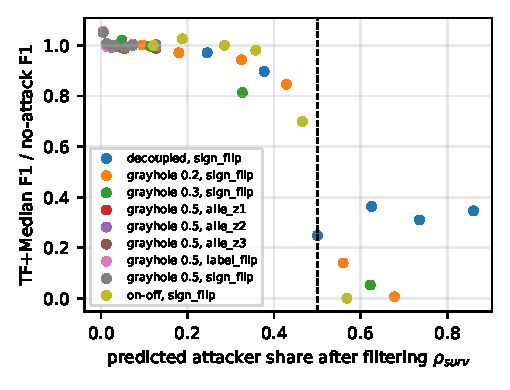
\includegraphics[width=0.9\columnwidth]{figs/fig_phase.pdf}
\caption{Relative F1 of TF+Median (F1 over the no-attack F1 of the same network) versus $\rsurv$ predicted
by~\eqref{eq:surv} from measured $\beta$, $\gamma$ and $\rho$, for 56 settings (attacker type, poisoning, $\rho$; settings whose no-attack F1 is below 0.5 are omitted).}
\label{fig:phase}
\end{figure}

Fig.~\ref{fig:phase} plots, for every setting with a learnable task, the relative F1 of TF+Median against $\rsurv$ computed from the measured
$\beta$ and $\gamma$. All 56 points fall on the predicted side of $\rsurv = 1/2$: the 48 settings with
$\rsurv < 0.5$ keep at least 70\% of the no-attack F1 (43 of them at least 97\%), and all 8 with $\rsurv > 0.5$
collapse to 0--36\%. The breakdown of a trust-filtered robust rule is predictable from two rates
that can be measured on the network.

\subsection{Ablation}

\begin{table}[t]
\caption{Filter ablation, sign-flip, $p_d = 0.5$: TF+Median F1 and filter rates over $\rho = 20$--70\%.
Static trust uses the whole run, including the future (an upper bound).}
\label{tab:abl}
\centering
\setlength{\tabcolsep}{3pt}
\begin{tabular}{lccccc}
\toprule
Variant & 50\% & 60\% & 70\% & $\beta$ & $\gamma$\\
\midrule
Mixture, $W = 10$~s (ours) & 0.91 & 0.97 & 0.97 & 0.05--0.06 & 0.08--0.12\\
Otsu threshold~\cite{otsu1979} & 0.91 & 0.96 & 0.77 & 0.03--0.04 & 0.55--0.76\\
No filter (= median) & 0.39 & 0.01 & 0.00 & 1 & 0\\
$W = 5$~s / $W = 20$~s & 0.91 & 0.96 & 0.97 & 0.04--0.07 & 0.06--0.11\\
Static trust (oracle) & 0.91 & 0.97 & 0.96 & 0.00 & 0.00--0.08\\
\bottomrule
\end{tabular}
\end{table}

Table~\ref{tab:abl} varies one choice at a time. Otsu's threshold rejects as few attackers as the mixture but cuts
inside the honest mode: it rejects 55--76\% of honest vehicles, leaves about nine clients per round, and TF+Median
fails in one of five seeds at 70\%. Without rejection, TF+Median is plain median and collapses from 50\%, and the
trust-weighted mean alone fails from 40\%, so the gain comes from rejection, not weighting. Windows of 5--20~s give
the same result, and the 10~s windowed filter already matches trust computed from the whole run.

\subsection{Failure modes}

\begin{figure*}[t]
\centering
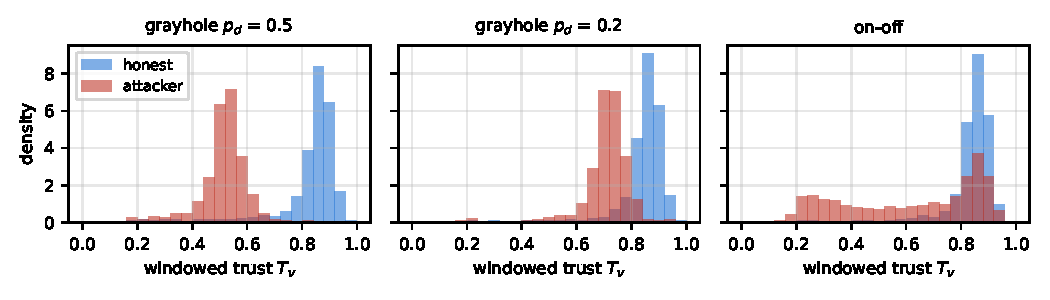
\includegraphics[width=0.85\textwidth]{figs/fig_trust.pdf}
\caption{Windowed trust of honest vehicles and attackers ($\rho = 0.3$, 5 seeds, every 5~s). Strong grayholes form a
separate mode; weak grayholes overlap the honest mode; on-off attackers spread across the range.}
\label{fig:trust}
\end{figure*}

\begin{table}[t]
\caption{Harder attackers, sign-flip (F1, mean of 5 seeds; $\rho$ = 40 / 50 / 60 / 70\%).}
\label{tab:fail}
\centering
\setlength{\tabcolsep}{2.5pt}
\begin{tabular}{llc}
\toprule
Attacker & Quantity & 40 / 50 / 60 / 70\%\\
\midrule
\multirow{4}{*}{grayhole, $p_d = 0.3$} & ceiling & 0.86 / 0.92 / 0.94 / 0.96\\
& $\beta$ & 0.18 / 0.11 / 0.29 / 0.67\\
& TF+Median & 0.86 / 0.92 / 0.77 / 0.05\\
& TF+Krum & 0.81 / 0.91 / 0.91 / 0.82\\
\midrule
\multirow{4}{*}{grayhole, $p_d = 0.2$} & ceiling & 0.77 / 0.86 / 0.90 / 0.91\\
& $\beta$ & 0.66 / 0.70 / 0.80 / 0.86\\
& TF+Median & 0.73 / 0.73 / 0.13 / 0.01\\
& TF+Krum & 0.72 / 0.79 / 0.82 / 0.69\\
\midrule
\multirow{4}{*}{on-off (10 s / 20 s)} & ceiling & 0.71 / 0.78 / 0.85 / 0.88\\
& $\beta$ & 0.54 / 0.51 / 0.53 / 0.54\\
& TF+Median & 0.71 / 0.76 / 0.59 / 0.00\\
& TF+Krum & 0.72 / 0.77 / 0.77 / 0.79\\
\midrule
\multirow{3}{*}{\shortstack[l]{on-off, memory\\60 s}} & $\beta$ & 0.18 / 0.17 / 0.18 / 0.20\\
& TF+Median & 0.71 / 0.77 / 0.84 / 0.27\\
& TF+Krum & 0.72 / 0.76 / 0.80 / 0.84\\
\midrule
\multirow{3}{*}{\shortstack[l]{on-off, memory\\60 s + warm-up 30 s}} & $\beta$ & -- / 0.08 / 0.07 / 0.09\\
& TF+Median & -- / 0.77 / 0.84 / 0.88\\
& TF+Krum & -- / 0.77 / 0.80 / 0.86\\
\midrule
\multirow{3}{*}{decoupled poisoners} & $\beta$ & 0.91 / 0.91 / 0.90 / 0.90\\
& $\gamma$ & 0.39 / 0.45 / 0.52 / 0.66\\
& best rule & 0.73 / 0.43 / 0.34 / 0.33\\
\bottomrule
\end{tabular}
\end{table}

The filter can only reject what the watchdog separates (Fig.~\ref{fig:trust}). \textbf{Weak grayholes}
($p_d = 0.2$--0.3) overlap honest vehicles that lose overhearings to collisions, so $\beta$ grows with $\rho$
(Table~\ref{tab:fail}) and TF+Median collapses where $\rsurv$ crosses one half (60--70\%); TF+Krum degrades gracefully
(0.69--0.91) because the sign-flipped updates that pass remain outliers. \textbf{On-off grayholes} keep a high windowed
trust half of the time ($\beta \approx 0.5$): TF and TF+Median collapse once $\rsurv > 1/2$, TF+Krum holds. A trust
memory of 60~s keeps an attacker suspect through its honest phase and cuts $\beta$ to 0.12--0.20 (at a $\gamma$ of
0.10--0.19); TF+Median then holds to 60\%, but at 70\% it still fails in three of five seeds although the pooled
$\rsurv \approx 0.34$. A 30~s warm-up removes these failures: $\beta$ falls to 0.07--0.09 and TF+Median reaches
0.77/0.84/0.88 at 50/60/70\%, all five seeds at 70\% between 0.84 and 0.90 (ceiling 0.88). A 30~s memory is weaker
than 60~s and 90~s is no better, a 60~s warm-up adds nothing over 30~s, and trust over the whole past dilutes bursts
($\beta = 0.16$ at 70\% even with warm-up).
\textbf{Decoupled poisoners}, which forward honestly, pass the filter ($\beta \approx 0.9$) while the honest-training
grayholes are rejected, so the poisoner share among kept updates \emph{rises}; all rules fail from 40\%. A
network-layer filter helps only when network and model misbehaviour come from the same vehicles.

\subsection{The detection transient}
\label{sec:perround}

Why does the pooled condition miss the on-off failures? For 1{,}260 TF+Median runs (setting, seed, fold) of the
sign-flip and ALIE settings, the ablation and the harder attackers, we computed the attacker share among accepted updates in every round. The pooled test $\rsurv \ge 1/2$ classifies 96.3\%
of the runs correctly (collapse: final F1 below half the ceiling) but misses 45 of 101 collapses. These share one
pattern: attackers are the majority of the accepted updates in the first rounds, before the watchdog has caught them,
and median aggregation drives the model into a state that the remaining honest-majority rounds do not repair. With
on-off attackers at 70\% and a 60~s memory, attackers hold 62--70\% of round 1 and a majority in about four of the
first five rounds; one seed recovers at round 15, the others never. Persistent grayholes are caught within one or two
rounds and the model recovers at once (F1 0.95 from round 3). Adding ``attacker majority in at least four of the first
five rounds'' to the pooled test raises the accuracy to 98.3\% (18 misses, 4 false alarms). Rejecting never-observed
vehicles does not help, because on-off attackers have been observed, in their honest phase. Robustness thus needs
$\rsurv < 1/2$ after the detection transient, and an observation period longer than the watchdog needs to see a burst.

% =====================================================================================
\section{Discussion and Limitations}
% =====================================================================================

\textbf{Why FL if trust flags attackers?} The filter needs neighbour reports aggregated over a window and acts only on
observed vehicles; the learned detector runs on each vehicle's own per-second features and generalises to vehicles
not yet scored. Both use network features, so applying the filter to an FL task with different inputs (e.g.,
misbehaviour detection from position messages) is the natural next step.

\textbf{Overhead.} Fitting the mixture takes 2--5~ms per round for 50 to 5{,}000 vehicles, the memory is a minimum over
about a dozen stored windows per vehicle, and the watchdog is passive overhearing with a table lookup. The real costs
are participation (updates lost to $\gamma$, 10--12\% even without attackers, and to the warm-up) and the reports,
about a dozen counters per vehicle per second.

\textbf{Limitations.} The radio is a unit disk and the road a ring rather than a SUMO trace, at 20--30~m/s in one
direction; higher relative speeds shorten contacts and will raise $\gamma$. Every vehicle joins every round, so the
round-level attacker share is set directly rather than produced by coverage and uploads. Five seeds per setting give
95\% intervals of about $\pm 0.01$--0.03 for the trust-filtered rules; collapsing rules are bimodal across seeds. Attackers do not forge route replies. The
watchdog assumes promiscuous overhearing. An on-off attacker whose honest phase exceeds the memory regains trust, at
the price of dropping less. Final-model F1 hides the transient: models taken during the first rounds can be poisoned.

% =====================================================================================
\section{Conclusion}
% =====================================================================================

Network-layer trust keeps Byzantine-robust FL working when attackers become a local or temporary majority of a
round, and costs no accuracy when they are rare. With watchdog trust, a label-free mixture threshold and a sliding
window, trust-filtered rules stay at the no-attack F1 up to a 70\% attacker share under sign-flip, label-flip and ALIE
poisoning, while every unfiltered rule fails against at least one of them. The breakdown point becomes
$(1-\gamma)/(1-\gamma+\beta)$, a function of two rates measurable on the network, and $\rsurv < 1/2$ predicted survival
in all 56 settings we tested. The defence ends where the watchdog cannot see: weak grayholes erode the
separation, on-off grayholes need slow trust recovery and an observation period, and honest-forwarding poisoners evade
the filter and are amplified by it.

\bibliographystyle{IEEEtran}
\bibliography{refs}

\end{document}
